\documentclass[a4paper, 10pt, twoside, notitlepage]{article}
% idioma
\usepackage[spanish]{babel}
\usepackage[utf8x]{inputenc}
\usepackage{graphicx}
\usepackage{multirow} % para las tablas

% graficos
%\usepackage[pdftex]{graphicx}
%\usepackage{wrapfig}

\usepackage{listings}
\lstset{language=C,basicstyle=\small,tabsize=3}

%\usepackage{epic,eepic}
% estilo
\usepackage[footnotesize]{caption}
\usepackage[outer=2cm,inner=4cm,top=2cm,bottom=2cm]{geometry}
\usepackage{fancyhdr}
\usepackage{lipsum}
\usepackage{pdfpages}

\usepackage{color,hyperref}
\definecolor{black}{rgb}{0.0,0.0,0.0}
\definecolor{darkblue}{rgb}{0.0,0.0,0.3}

\hypersetup{colorlinks,breaklinks,
            linkcolor=black,urlcolor=darkblue,
            anchorcolor=darkblue,citecolor=darkblue}

% matematica
\usepackage{amsmath} \usepackage{amsfonts} \usepackage{amssymb}

\title{\textbf{Trabajo Práctico 1:\\Programación en MIPS} \\}

\author{ \\
         Ronnie Del Pino Cárdenas, \textit{Padrón 93575} \\
          \texttt{ delpinor@gmail.com }       \\
		  [2.5ex]
         Emiliano Vega, \textit{Padrón 76676}     \\
          \texttt{emiliano.vega@mail.com}                      \\ 
		  [2.5ex]
	 Romina Casal, \textit{Padrón 86429} \\
          \texttt{casal.romina@gmail.com}                      \\ 
		  [2.5ex]
		 \\
         \normalsize{2do. Cuatrimestre de 2019}            \\
         \normalsize{86.37 / 66.20 Organización de Computadoras $-$ Práctica Jueves} \\
         \normalsize{Facultad de Ingeniería, Universidad de Buenos Aires} 
       }

\date{}

\begin{document}

\maketitle
% \thispagestyle{empty}   % quita el número en la primer página

% \newpage
% Es un breve resumen de lo que vamos a leer con mayor profundidad en las secciones posteriores, tiene que resaltar lo más importante.
\begin{abstract}
El presente trabajo práctico nos permitió realizar una comparativa entre la performance de dos implementaciones de un programa en C basado en el algoritmo "La hormiga artista" del trabajo práctico anterior en varios niveles de optimización y reemplazando dos funciones clave a código MIPS. Para el análisis se utilizó el programa /usr/bin/time que nos da los tiempos de ejecución resultante.
\end{abstract}

% \tableofcontents
% 
% \newpage
% 

\pagestyle{fancy}
\fancyhead{}
\fancyfoot{}
\renewcommand{\sectionmark}[1]{\markright{\thesection\ #1}}
\renewcommand{\headrulewidth}{0.4pt}
%\renewcommand{\footrulewidth}{0.4pt}
\fancyhead[LE]{\nouppercase \rightmark}
\fancyhead[RE, LO]{\bf \thepage}
\fancyhead[RO]{\nouppercase \rightmark}
\fancyfoot[C]{ }
\maketitle
%genera el indice - compilar dos veces
\setcounter{page}{1}
% \tableofcontents
% \newpage

\parskip 7.2pt
%Distinto al resumen, se dice cual es el objetivo principal y se hace un resumen de cada parte que aparece a continuación. 
\section{Introducción}
Para la realización de las pruebas se ha creado un Makefile adaptado que permite compilar las versiones tp1\_if y tp1\_tables en los niveles 0, 1, 2 y 3 de optimización que ofrece gcc, además de las versiones con las funciones new\_orientation y move\_forward en código assembly.\\
Se realizará la ejecución de varias opciones de iteraciones con estas versiones para comparar los distintos tiempos de ejecución y observar la tasa de mejora lograda.\\

%Una de las secciones más importantes del informe. Aquí se explaya todo lo realizado, problemas encontrados y soluciones propuestas con variantes y métricas.

\newpage

\section{Proceso de Compilación}
Se adaptó el archivo makefile provisto por la cátedra para generar los ejecutables con las distintas opciones de optimización para el código integralmente en C.\\

\begin{itemize} 
\item[] \textbf{make all\_tp1\_c}: Crea los ejecutables tp1\_if\_opt0, tp1\_if\_opt1, tp1\_if\_opt2, tp1\_if\_opt3 para la versión con jumps en los distintos niveles de optimización, y tp1\_tables\_opt0, tp1\_tables\_opt1, tp1\_tables\_opt2, tp1\_tables\_opt3 para la versión con tables.
\item[] \textbf{make tp1\_tables\_asm}: Crea el ejecutable tp1\_tables\_asm para la versión con table que tiene las funciones new\_orientation y move\_forward en assembly.
\item[] \textbf{make tp1\_if\_asm}: Crea el ejecutable tp1\_if\_asm para la versión con jumps que tiene las funciones new\_orientation y move\_forward en assembly.
\end{itemize}
Creamos un archivo script pruebas.sh que usando \textbf{/usr/bin/time} cuenta el tiempo de ejecución de cada prueba y guarda los resultados en un archivo \textbf{test\_result.txt}
Con los valores obtenidos en este archivo se crearon gráficas comparativas de tiempo de ejecución en función de la cantidad de iteraciones.\\

Por ejemplo, la línea:

\scriptsize
\begin{verbatim}
/usr/bin/time --output=test_result.txt -a -f "%E\treal\t%U\tuser\t%S\tsys" ./tp1_if_opt0 -g 1000x1000 -p RGBW -r LLLL -t $((10000)) > /dev/null
\end{verbatim}
\normalsize
Escribirá el siguiente resultado en \textbf{test\_result.txt}

\scriptsize
\begin{verbatim}
0:11.39	real	11.14	user	0.03	sys
\end{verbatim}
\normalsize

De esa medición usaremos el tiempo real de ejecución obtenido para las comparaciones.\\
NOTA: Es probable que sea necesario instalar en la VM ejecutada con QEMU el programa time que tiene opciones adicionales que el homónimo que trae por defecto no permite usar.\\

\newpage
\section{Desarrollo}
\normalsize
ACA ESCRIBIMOS SOBRE LAS DECISIONES DE DESARROLLO \\
\\

\newpage
\section{Resultados obtenidos}
Ejecutamos el script \textbf{pruebas.sh} y arroja los siguientes resultados que exporta al archivo \textbf{test\_result.txt}:

\scriptsize
\begin{verbatim}
Pruebas TP1
Grafico de iteraciones
tp1_if - optimizacion 0
0:11.39	real	11.14	user	0.03	sys
0:12.41	real	12.35	user	0.04	sys
0:12.19	real	12.16	user	0.02	sys
0:18.53	real	18.50	user	0.01	sys
1:19.81	real	79.50	user	0.04	sys
11:41.06	real	700.63	user	0.03	sys
tp1_if - optimizacion 1
0:10.25	real	10.20	user	0.03	sys
0:10.66	real	10.62	user	0.02	sys
0:10.18	real	10.14	user	0.03	sys
0:15.36	real	15.30	user	0.04	sys
0:50.10	real	50.03	user	0.02	sys
6:47.14	real	406.88	user	0.02	sys
tp1_if - optimizacion 2
0:11.16	real	11.12	user	0.03	sys
0:11.11	real	11.08	user	0.02	sys
0:12.02	real	11.96	user	0.04	sys
0:18.66	real	18.62	user	0.02	sys
0:47.17	real	47.12	user	0.02	sys
6:26.73	real	386.48	user	0.03	sys
tp1_if - optimizacion 3
0:09.87	real	9.83	user	0.02	sys
0:09.99	real	9.95	user	0.02	sys
0:11.56	real	11.52	user	0.02	sys
0:14.15	real	14.12	user	0.01	sys
0:45.25	real	45.21	user	0.00	sys
6:00.04	real	359.80	user	0.03	sys
tp1_tables - optimizacion 0
0:09.61	real	9.57	user	0.01	sys
0:11.39	real	11.37	user	0.00	sys
0:12.67	real	12.63	user	0.02	sys
0:22.76	real	22.71	user	0.03	sys
1:47.64	real	107.54	user	0.03	sys
17:00.54	real	1019.67	user	0.05	sys
tp1_tables - optimizacion 1
0:08.93	real	8.89	user	0.02	sys
0:10.60	real	10.56	user	0.02	sys
0:12.15	real	12.11	user	0.02	sys
0:14.79	real	14.74	user	0.03	sys
0:55.26	real	55.21	user	0.01	sys
8:04.03	real	483.73	user	0.02	sys
tp1_tables - optimizacion 2
0:11.35	real	11.31	user	0.02	sys
0:10.24	real	10.19	user	0.04	sys
0:12.67	real	12.61	user	0.03	sys
0:16.59	real	16.55	user	0.02	sys
0:59.45	real	59.38	user	0.03	sys
10:28.80	real	628.41	user	0.04	sys
tp1_tables - optimizacion 3
0:09.76	real	9.71	user	0.03	sys
0:11.14	real	11.10	user	0.02	sys
0:10.42	real	10.37	user	0.03	sys
0:17.49	real	17.45	user	0.02	sys
0:59.53	real	59.45	user	0.03	sys
8:16.94	real	496.64	user	0.02	sys
tp1_if - assembly
0:10.65	real	10.62	user	0.01	sys
0:11.28	real	11.24	user	0.02	sys
0:11.25	real	11.22	user	0.01	sys
0:24.52	real	24.47	user	0.02	sys
1:31.24	real	91.13	user	0.03	sys
14:27.08	real	866.43	user	0.04	sys
tp1_tables - assembly
0:11.83	real	11.80	user	0.01	sys
0:10.47	real	10.42	user	0.03	sys
0:13.32	real	13.26	user	0.03	sys
0:19.97	real	19.92	user	0.03	sys
1:56.73	real	116.64	user	0.01	sys
14:57.11	real	896.46	user	0.05	sys
\end{verbatim}

\newpage
\normalsize
Con los datos obtenidos en las pruebas realizamos dos gráficos comparativas entre las distintas optimizaciones y la versión con funciones en assembly para cada implementación que reflejan el tiempo de ejecución en función de la cantidad de iteraciones:

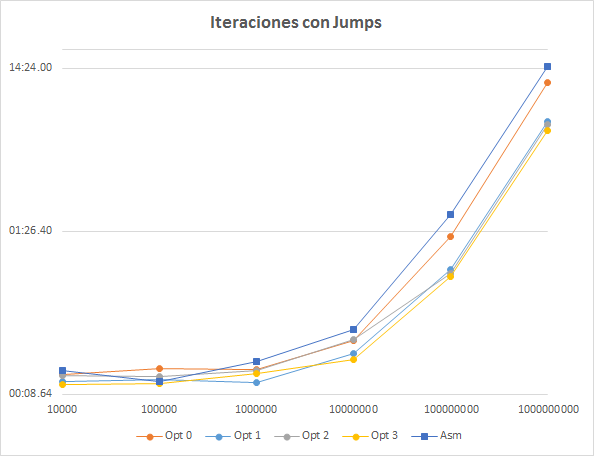
\includegraphics[scale=0.9]{chart1.png} 

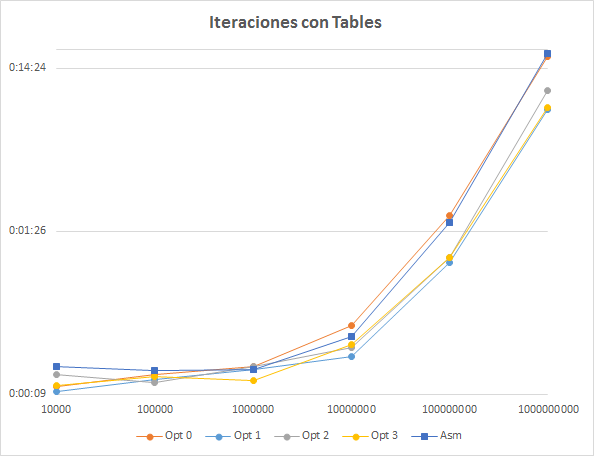
\includegraphics[scale=0.9]{chart2.png} 

\newpage
En ellos observamos dos tendencias:\\
En la implementación con jumps, las mediciones nos muestran que la implementación con las funciones \textbf{new\_orientation} y \textbf{move\_forward} en assembly tuvieron una performance inferior que las contrapartidas en C, incluso la compilada con la opción -O0.
Otra cosa que podemos observar es que de la optimización con opción -O0 a -O1 ya una mejora más significativa que la obtenida entre las compilaciones hechas con opciones -O1, -O2 y -O3.\\
En la implementación con tables, se observa que la implementación con las funciones en assembly mostró un mejor resultado que la opción -O0, pero aún menos performante que con la opción -O1. Además, entre las opciones -O1 y -O2 hay una diferencia de performance mayor que entre las análogas de la implementación con jumps. Luego, entre las compilacionese con -O2 y -O3 sí coincide la tendencia a mostrar una mejora poco significativa.

\newpage

\section{Conclusión}
<< CONCLUSIONES FINAL >> 


\vspace{.5cm}
%Referencias o recursos utilizados durante la investigación para la resolución del trabajo práctico 
\begin{thebibliography}{5}
 \bibitem{} Profiling and Timing Code
.\\ \url{https://jakevdp.github.io/PythonDataScienceHandbook/01.07-timing-and-profiling.html}.
 \bibitem{} C to MIPS compiler
.\\ \url{http://reliant.colab.duke.edu/c2mips/}.

\end{thebibliography}

\clearpage

\part{Apéndice}
\appendix

\normalsize
\section{Código fuente}\label{sec:codigofuente}
\subsection{ant\_engine\_jumps.S}
\begin{lstlisting}
#include <regdef.h>
#define ON 0
#define OS 1
#define OE 2
#define OW 3


.data
ime: .asciiz "TP1 2Q2019: Implement me!"

.text
.align 2
.globl new_orientation
.ent new_orientation

new_orientation:
#    la a0, ime
#    jal doPanic
#armo stack
	subu	sp, sp, 24
	sw	ra, 16(sp)
	sw	fp, 12(sp)
	sw	gp, 8(sp)
	move 	fp, sp

	# guardo parametros
	sw	a0, 0(sp)	# orientation
	sw	a1, 4(sp)	# rule
	# cargo parametros en registros
	move	t0, a0
	move	t1, a1
	
	# orientacion?
	
norte:	bne	t0, 0, sur
	bne	t1, zero, norte_derecha	# RL = 0
	addi	t2, zero, 3			# OW = 3
	j	return_value
norte_derecha:
	addi	t2, zero, 2			# OE = 2
	j	return_value
sur:	bne	t0, 1, este
	bne	t1, zero, sur_derecha
	addi	t2, zero, 2
	j	return_value
sur_derecha:
	addi	t2, zero, 3
	j	return_value
este:	bne	t0, 2, oeste
	bne	t1, zero, este_derecha
	addi	t2, zero, 0			# ON = 0
	j	return_value
este_derecha:
	addi	t2, zero, 1			# OS = 1
	j	return_value
			
oeste:	bne	t1, zero, oeste_derecha
	addi	t2, zero, 1
	j	return_value
oeste_derecha:
	addi	t2, zero, 0
	
return_value:
	# return new orientation
	move	v0, t2
			
	#borro stack
	lw	gp, 8(sp)
	lw	fp, 12(sp)
	lw	ra, 16(sp)
	addu	sp, sp, 24
	jr	ra


.end new_orientation

.text
.align 2
.globl move_forward
.ent move_forward
move_forward:
	#    la a0, ime
	#   jal doPanic
	# allocate stack frame(SRA=8 LTA=0 ABA=0)
	addi	sp, sp, -8
	sw		fp, 4(sp)
	sw		gp, 0(sp)
	move 	fp, sp

	# load struct ant_t
	lw		t0, 0(a0)			# x
	lw		t1, 4(a0)			# y
	lw		t2, 8(a0)			# o
	# switch statement
	bne		t2, ON, case_south
	# adjust(&ant->y, ant->y - 1, height);
	addi	t1, t1, -1		# ant->y - 1
	div		t1, a2			# ant->y / heigth
	mfhi	t5					# remainder moved into t5
	sw		t5, 4(a0)			# &ant->y
	j		done
case_south:
	bne		t2, OS, case_east
	addi	t1, t1, 1			# ant->y + 1
	div		t1, a2			# ant->y / height
	mfhi	t5					# remainder moved into t5
	sw		t5, 4(a0)			# &ant->y
	j		done
case_east:
	bne		t2, OE, case_west
	addi	t0, t0, 1			# ant->x + 1
	div		t0, a1				# ant->x / width
	mfhi	t5					# remainder moved into t5
	sw		t5, 0(a0)			# &ant->x
	j		done
case_west:
	#bne		t2, OW, case_default
	addi	t0, t0, -1		# ant->x + 1
	div		t0, a1			# ant->x / width
	mfhi	t5					# remainder moved into t5
	sw		t5, 0(a0)			# &ant->x
	j		done
done:
	lw		fp, 4(sp)
	lw		gp, 0(sp)
	addiu	sp, sp, 8
	move	v0, a0			# Save the return value in v0
	jr		ra
.end move_forward

\end{lstlisting}

\normalsize
\subsection{ant\_engine\_tables.S}
\begin{lstlisting}
#include <regdef.h>
#define ON 0
#define OS 1
#define OE 2
#define OW 3
.data
ime: .asciiz "TP1 2Q2019: Implement me!"
rotation_rules:	.word	3, 2, 2, 3, 0, 1, 1, 0
allowed_forward: .word 0, 1, 2, 3		# steps
.text
.align 2
.globl new_orientation
.ent new_orientation

new_orientation:
#    la a0, ime
#    jal doPanic
	#armo stack
	subu	sp, sp, 24
	sw	ra, 16(sp)
	sw	fp, 12(sp)
	sw	gp, 8(sp)
	move 	fp, sp

	# guardo parametros
	sw	a0, 0(sp)	# orientation
	sw	a1, 4(sp)	# rule
	
	# cargo parametros en registros
	# y calculo indice en el array
	mul	t0, a0, 8	# indice orientation x 4bytes = word
	mul	t1, a1, 4
	add	t0, t0, t1
	la	t2, rotation_rules(t0)

	# return new orientation
	lw	v0, (t2)

	#borro stack
	lw	gp, 8(sp)
	lw	fp, 12(sp)
	lw	ra, 16(sp)
	addu	sp, sp, 24
	jr	ra
    
.end new_orientation

.text
.align 2
.globl move_forward
.ent move_forward
move_forward:
    #la a0, ime
    #jal doPanic
    addi	sp, sp, -32			#allocate stack frame(SRA=16 LTA=16 ABA=0)
    sw		ra, 24(sp)
    sw		fp, 20(sp)
    sw		gp, 16(sp)
    sw		a2, 12(sp)			# relevants_bouds[0] = height
    sw		a2, 8(sp)				# relevants_bouds[1] = height
    sw		a1, 4(sp)				# relevants_bouds[2] = width
    sw		a1, 0(sp)				# relevants_bouds[3] = width
    lw		t3, 8(a0)				# load ant_t->o = index
    sll		t3, t3, 2				# index*4
    add		t4, t3, sp			# base + index*4
    lw		t4, 0(t4)				# = bound
    la		t5, allowed_forward	# base array address
    add		t5, t5, t3			# base + index*4
	lw		t5, 0(t5)				# = step_fun
	bne		t5, ON, step_south		# step_north
	lw		t6, 4(a0)				# ant->y
	addi	t6, t6, -1			# ant->y - 1
	div		t6, t4				# ant->y / height
	mfhi	t6						# remainder moved into t6
	sw		t6, 4(a0)				# &ant->y
	j		done
step_south:
	bne		t5, OS, step_east
	lw		t6, 4(a0)				# ant->y
	addi	t6, t6, 1				# ant->y + 1
	div		t6, t4				# ant->y / height
	mfhi	t6						# remainder moved into t6
	sw		t6, 4(a0)				# &ant->y
	j		done
step_east:
	bne		t5, OE, step_west
	lw		t6, 0(a0)				# ant->x
	addi	t6, t6, 1				# ant->x + 1
	div		t6, t4				# ant->x / width
	mfhi	t6						# remainder moved into t6
	sw		t6, 0(a0)				# &ant->x
	j		done
step_west:
	lw		t6, 0(a0)				# ant->x
	addi	t6, t6, -1			# ant->x - 1
	div		t6, t4				# ant->x / width
	mfhi	t6						# remainder moved into t6
	sw		t6, 0(a0)				# &ant->x
	j		done
done:
	lw		ra, 24(sp)
    lw		fp, 20(sp)
    lw		gp, 16(sp)
    addi	sp, sp, 32
    move	v0, a0
    jr		ra
.end move_forward
#fin
\end{lstlisting}

\newpage
\normalsize
\section{Diagramas de stacks}\label{sec:diagstacks}

\subsection{ant\_engine\_jumps.S}

\begin{table}[htp]
\centering
\begin{tabular}{cccllll}
\multicolumn{3}{c}{\textbf{new\_orientation}}                                                                                &                       & \multicolumn{3}{c}{\textbf{move\_forward}}                                                                                  \\ \cline{1-3} \cline{5-7} 
\multicolumn{1}{|l|}{\textbf{Sección}}     & \multicolumn{1}{c|}{\textbf{Variable}} & \multicolumn{1}{c|}{\textbf{Posición}} & \multicolumn{1}{l|}{} & \multicolumn{1}{c|}{\textbf{Sección}}     & \multicolumn{1}{c|}{\textbf{Variable}} & \multicolumn{1}{c|}{\textbf{Posición}} \\ \cline{1-3} \cline{5-7} 
\multicolumn{1}{|c|}{\multirow{4}{*}{SRA}} & \multicolumn{1}{c|}{-}                 & \multicolumn{1}{c|}{20}                & \multicolumn{1}{l|}{} & \multicolumn{1}{c|}{\multirow{2}{*}{SRA}} & \multicolumn{1}{c|}{fp}                & \multicolumn{1}{c|}{4}                 \\ \cline{2-3} \cline{6-7} 
\multicolumn{1}{|c|}{}                     & \multicolumn{1}{c|}{ra}                & \multicolumn{1}{c|}{16}                & \multicolumn{1}{l|}{} & \multicolumn{1}{c|}{}                     & \multicolumn{1}{c|}{gp}                & \multicolumn{1}{c|}{0}                 \\ \cline{2-3} \cline{5-7} 
\multicolumn{1}{|c|}{}                     & \multicolumn{1}{c|}{fp}                & \multicolumn{1}{c|}{12}                &                       &                                           &                                        &                                        \\ \cline{2-3}
\multicolumn{1}{|c|}{}                     & \multicolumn{1}{c|}{gp}                & \multicolumn{1}{c|}{8}                 &                       &                                           &                                        &                                        \\ \cline{1-3}
\multicolumn{1}{|c|}{\multirow{2}{*}{LTA}} & \multicolumn{1}{c|}{orientation}       & \multicolumn{1}{c|}{4}                 &                       &                                           &                                        &                                        \\ \cline{2-3}
\multicolumn{1}{|c|}{}                     & \multicolumn{1}{c|}{rule}              & \multicolumn{1}{c|}{0}                 &                       &                                           &                                        &                                        \\ \cline{1-3}
\end{tabular}
\end{table}

\subsection{ant\_engine\_tables.S}

\begin{table}[htp]
\centering
\begin{tabular}{cccllll}
\multicolumn{3}{c}{\textbf{new\_orientation}}                                                                                &                       & \multicolumn{3}{c}{\textbf{move\_forward}}                                                                                  \\ \cline{1-3} \cline{6-7} 
\multicolumn{1}{|c|}{\textbf{Sección}}     & \multicolumn{1}{c|}{\textbf{Variable}} & \multicolumn{1}{c|}{\textbf{Posición}} & \multicolumn{1}{l|}{} & \multicolumn{1}{l|}{\textbf{Sección}}     & \multicolumn{1}{l|}{\textbf{Variable}} & \multicolumn{1}{l|}{\textbf{Posición}} \\ \cline{1-3} \cline{5-7} 
\multicolumn{1}{|c|}{\multirow{4}{*}{SRA}} & \multicolumn{1}{c|}{-}                 & \multicolumn{1}{c|}{20}                & \multicolumn{1}{l|}{} & \multicolumn{1}{l|}{\multirow{4}{*}{SRA}} & \multicolumn{1}{l|}{-}                 & \multicolumn{1}{l|}{28}                \\ \cline{2-3} \cline{6-7} 
\multicolumn{1}{|c|}{}                     & \multicolumn{1}{c|}{ra}                & \multicolumn{1}{c|}{16}                & \multicolumn{1}{l|}{} & \multicolumn{1}{l|}{}                     & \multicolumn{1}{l|}{ra}                & \multicolumn{1}{l|}{24}                \\ \cline{2-3} \cline{6-7} 
\multicolumn{1}{|c|}{}                     & \multicolumn{1}{c|}{fp}                & \multicolumn{1}{c|}{12}                & \multicolumn{1}{l|}{} & \multicolumn{1}{l|}{}                     & \multicolumn{1}{l|}{fp}                & \multicolumn{1}{l|}{20}                \\ \cline{2-3} \cline{6-7} 
\multicolumn{1}{|c|}{}                     & \multicolumn{1}{c|}{gp}                & \multicolumn{1}{c|}{8}                 & \multicolumn{1}{l|}{} & \multicolumn{1}{l|}{}                     & \multicolumn{1}{l|}{gp}                & \multicolumn{1}{l|}{16}                \\ \cline{1-3} \cline{5-7} 
\multicolumn{1}{|c|}{\multirow{2}{*}{LTA}} & \multicolumn{1}{c|}{orientation}       & \multicolumn{1}{c|}{4}                 & \multicolumn{1}{l|}{} & \multicolumn{1}{l|}{\multirow{4}{*}{LTA}} & \multicolumn{1}{l|}{a}                 & \multicolumn{1}{l|}{12}                \\ \cline{2-3} \cline{6-7} 
\multicolumn{1}{|c|}{}                     & \multicolumn{1}{c|}{rule}              & \multicolumn{1}{c|}{0}                 & \multicolumn{1}{l|}{} & \multicolumn{1}{l|}{}                     & \multicolumn{1}{l|}{b}                 & \multicolumn{1}{l|}{8}                 \\ \cline{1-3} \cline{6-7} 
                                           &                                        &                                        & \multicolumn{1}{l|}{} & \multicolumn{1}{l|}{}                     & \multicolumn{1}{l|}{c}                 & \multicolumn{1}{l|}{4}                 \\ \cline{6-7} 
                                           &                                        &                                        & \multicolumn{1}{l|}{} & \multicolumn{1}{l|}{}                     & \multicolumn{1}{l|}{d}                 & \multicolumn{1}{l|}{0}                 \\ \cline{5-7} 
\end{tabular}
\end{table}

\newpage
\section{Enunciado original}\label{sec:enunciado}
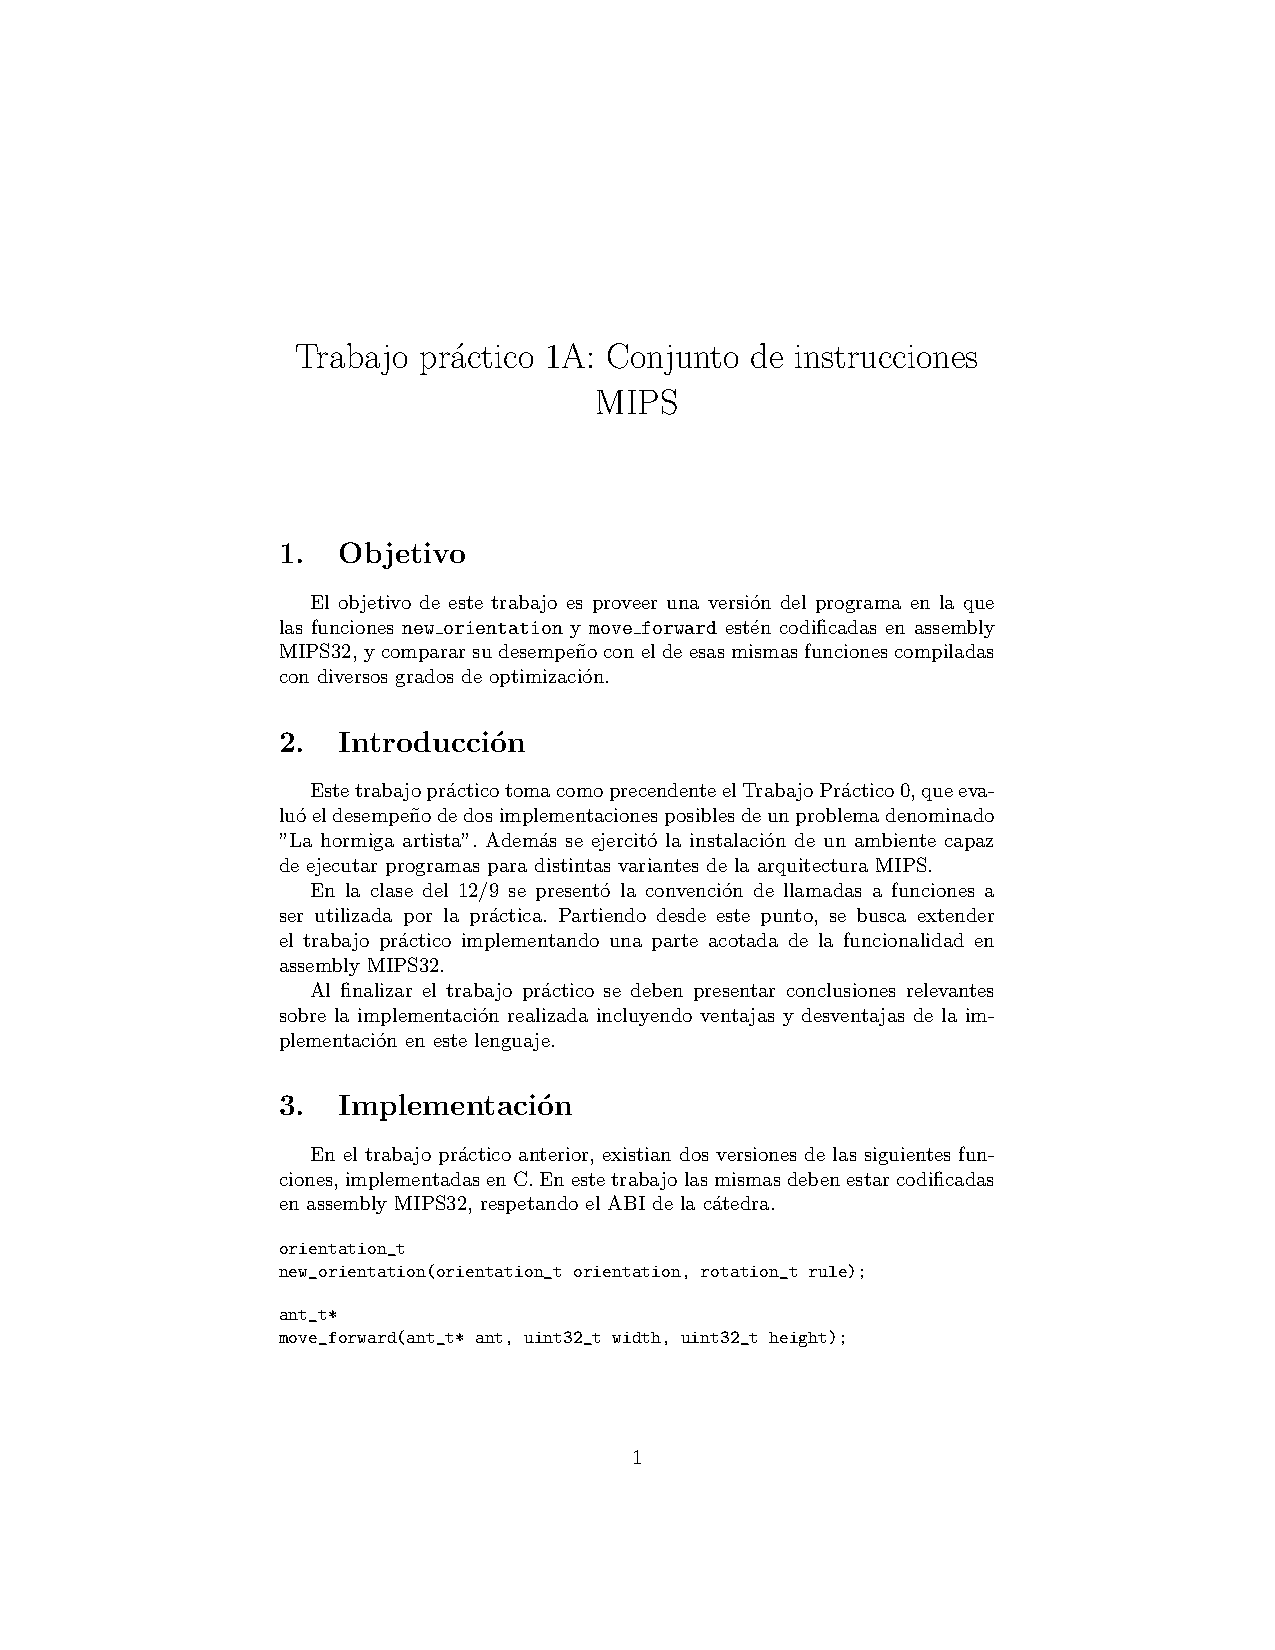
\includepdf[pages={-}]{enunciado.pdf}

\end{document}
